% This is samplepaper.tex, a sample chapter demonstrating the
% LLNCS macro package for Springer Computer Science proceedings;
% Version 2.20 of 2017/10/04
%
% Modifikace pro Data a znalosti: Radek Burget burgetr@fit.vutbr.cz
%
% Kódování dokumentu UTF-8

\documentclass[a4paper]{llncs}
\usepackage[english]{babel}
\usepackage[utf8]{inputenc}
\usepackage{makecell}
\usepackage{graphicx}
\usepackage{svg}

% Used for displaying a sample figure. If possible, figure files should
% be included in EPS format.
%
% If you use the hyperref package, please uncomment the following line
% to display URLs in blue roman font according to Springer's eBook style:
% \renewcommand\UrlFont{\color{blue}\rmfamily}


% Standardní české nadpisy. Zakomentujte nebo smažte, pokud píšete anglicky.
%\addto\captionsczech{\renewcommand\abstractname{Abstrakt.}}
%\addto\captionsczech{\renewcommand\keywordname{{\bf Klíčová slova:}}}
%\addto\captionsczech{\renewcommand\tablename{Tab.}}
%\addto\captionsczech{\renewcommand\figurename{Obr.}}
%\addto\captionsczech{\renewcommand\refname{Literatura}}

\begin{document}
%
\title{Project Thoth\,--\,A Recommendation Engine for Machine Learning Applications}
%
%
\author{Fridol\'in Pokorn\'y, Christoph G\"orn}

\institute{Red Hat Czech s.r.o., Purky\v{n}ova 99, 612 00 Brno\\
\email{\{fridolin,goern\}@redhat.com}}

\maketitle
\begin{abstract}
There has been seen a hype over the past years in AI and machine learning. Machine learning and AI applications are used in production systems which require significant effort to ensure applications behave correctly and are fully operational. In this paper we describe a recommendation system for AI and machine learning applications which use popular open source machine learning libraries. The described system, Thoth, is capable of storing observations based on which it predicts possible misbehavior in application, application assembling errors or issues when integrating application with other components in a deployment.
\keywords{machine learning \and artificial intelligence \and big data \and graph database \and data processing \and distributed systems \and Python}
\end{abstract}

\section{Introduction}

In this paper we present the designed platform that is a recommendation engine for applications and their dependency stacks. The main purpose of the designed system is to predict misbehavior in applications as well as how to prevent from them. The problematic of an application stack is described with a listing of possible issues that can arise when relying directly or indirectly on a logic that, in the end, create the resulting runnable application compound by libraries.

\section{Application Stack}

To build complex applications, there is often a need to create small building blocks that encapsulate required logic into an easy to access interface. These small units are often reusable and thus create a separate libraries used by libraries themselves as well as by the created application. The described dependency chaining creates direct or transitive requirements (also know as an application stack) for an application that is handled by a dependency management system in the given language ecosystem. Dependency management system hepls to resolve dependencies given the version range specified to meet required functionality offered by required dependencies.

Given the complexity in applications and their dependencies answering a question which dependencies in which versions are the best possible fit for available hardware in the given runtime environment is not trivial and requires knowledge about the language ecosystem used and behavioral characteristics of the successfully assembled application.

As applications evolve, it is not rare to see a broken application that does not assemble due to changes in libraries used, or simply breaks the expected behavior even without any visible notices. Having properly locked versions of libraries helps to solve issues in most cases, but this approach does not help to keep application always up-to-date with recent fixes in libraries used. An automated system Thoth, presented in the upcoming sections, answers and predicts which libraries in which versions are the most suitable ones for the given requirements saving computational and developer time and, moreover, learns from errors that create patterns already seen in other application stacks.

\subsection{Modelling Application Stacks in a Graph Database} \label{section_modelling_app_stacks}

Considering dependencies, their relations between each other, the whole application can be modeled in a graph database. We chosed JanusGraph graph database to be our data store for storing data in a graph form.

We model two main distinguishable information:

\begin{itemize}
  \item \emph{Ecosystem data itself}\,--\,how the given ecosystem looks like based on a declarative version range specification, what are dependencies between packages and observations like whether the given package is resolvable.
  \item \emph{Observations}\,--\,observations we gathered about packages and application stacks during continuous integration system (CI) or continuous delivery system (CD).
\end{itemize}

This data model connects data needed for creating recommendations for a user.

\subsection{Observations and Predictions}

To give recommendations to a user there is a need to aggregate data. Thoth for this purpose aggregates raw data mentioned in the section~\ref{section_modelling_app_stacks}. These data create a base for two core types of observations driving recommendations:

\begin{itemize}
  \item \emph{Package level data}\,--\,information gathered solely on package level. An example of such information can a fact that the given package is installable into the requested runtime environment.
  \item \emph{Application stack level data}\,--\,information about application stack assembling and errors that were found during application assembling in CI or negative feedback in the production environment on deployment or runtime (CD or directly user feedback).
\end{itemize}

These two fundamental observations are inputs for the scoring function which outputs the best possible application stack with fully locked down versions for deployment or an experimental application stack for gathering additional observations respecting new package releases or new environments.

\section{Thoth Architecture and Development}

Project Thoth runs on OpenShift to guarantee high horizontal scalability and high availability in case of failures. In some cases, there is a need to directly execute untrusted and potentially malicious code shipped within analyzed Python packages. For this purpose, there is done a restriction using OpenShift's Network Policy mechanism to restrict networking access. Also, OpenShift's namespaces help us with assigning resource quotas for application to restrict from DoS attacks and serve user requests asynchronously, if needed.

\begin{figure}[h!]
  \centering
  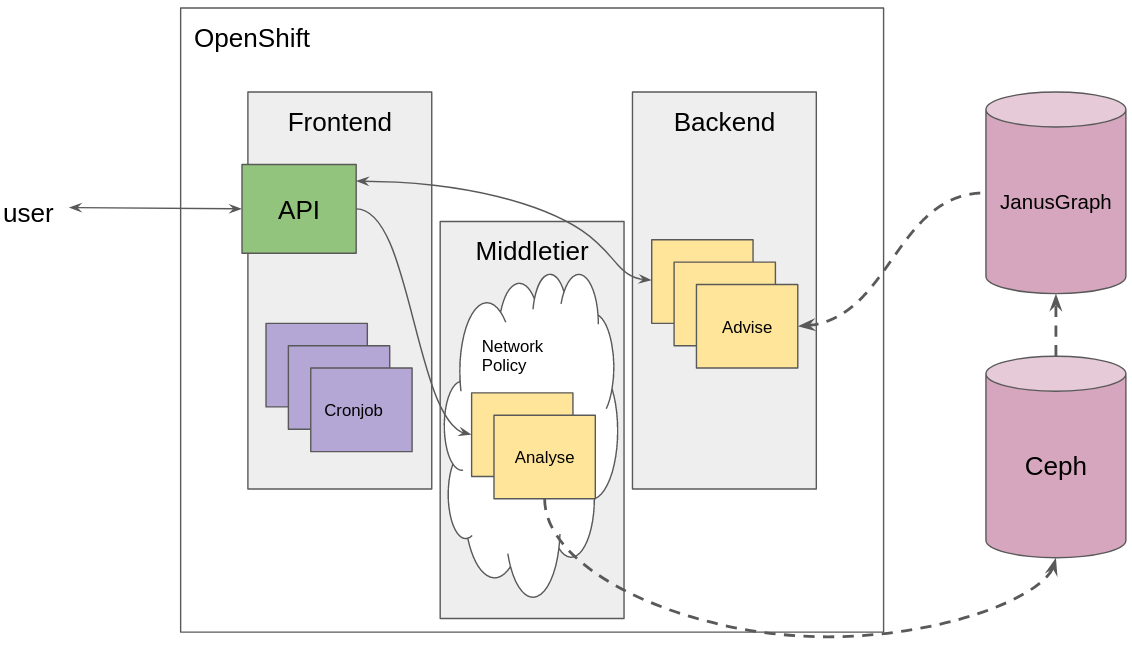
\includegraphics[width=1.0\textwidth]{fig/design.png}
  \caption{An architecture of Thoth.}
  \label{design}
\end{figure}

The deployment is separated into three namespaces. In the \emph{Frontnend} namespace there are available cronjobs, that perform periodic tasks ensuring the whole system is up-to-date, and a scalable API service that is the main interaction point for a user.

The \emph{Middletier} namespace is the restricted environment where all analyses are performed. Raw results are serialized into a JSON format and stored on an object storage Ceph~\cite{ref_ceph}. One of the cronjobs in the \emph{Frontend} namespace ensures all resutls are stored properly in the graph database. The database separation is needed due to security (possibly malicious software does not access production data in the JanusGraph) and to guarantee fully recoverable production graph database.

The last namespace called \emph{Backend} is used to guarantee SLA of the application for serving user requests. There is allocated a resource pool that is assigned for the recommendation engine itself.

\subsection{Lab}

As discovering new fields and ideas require experiments, project Thoth is designed of loosely coupled packages that, when assembled together, create a ready to deply Thoth but can also assemble an interactive experimental development environment using Jupyter Hub and its Jupyter Notebooks.

All experiments can be done in an interactive form that is sharable in the team using Jupyter notebooks. This allows experiments to be easily accommodated in production code.

\subsection{Bots\,--\,Junior Developers}

To automate every-days tasks, project Thoth comes with bots that ensure the project dependencies and Thoth's components are always up-to-date. If a component in the Thoth's architecture gets updated, a bot automatically updates all the relevant components. Moreover, if there is given a human review, another bot ensures the pull request is merged only if the change does not break existing parts of Thoth (CI/CD checks).

\section{Conclusion}

Project Thoth is open source and available on GitHub~\cite{ref_thoth}. It is written in the Python programming language to support popular Python machine learning and AI packages out of the box. The deployment is orchestrated by OpenShift~\cite{ref_openshift} to guarantee high horizontal scalability to serve high load of user requests as well as a separation needed for security. The whole system is exposed via an API endpoint where users can get recommendations for their machine learning and AI applications.

%
% ---- Bibliography ----
%
% BibTeX users should specify bibliography style 'splncs04'.
% References will then be sorted and formatted in the correct style.
%
% \bibliographystyle{splncs04}
% \bibliography{mybibliography}
%
\begin{thebibliography}{8}
\bibitem{ref_thoth}
Project Thoth on GitHub, \url{https://github.com/thoth-station/}. Last accessed 28 May 2018

\bibitem{ref_openshift}
OpenShift: Container Application Platform by Red Hat, \\ \url{https://www.openshift.com}. Last accessed 28 May 2018

\bibitem{ref_ceph}
Ceph: Homepage \url{https://www.ceph.com}. Last accessed 28 May 2018
\end{thebibliography}

%=============================================================================

%\bigskip
%\noindent \textbf{Poděkování:} Tento článek vznikl díky částečné podpoře projektů \dots

\end{document}
